\documentclass[a4paper]{article}
\usepackage[utf8]{inputenc}
\usepackage[russian,english]{babel}
\usepackage[T2A]{fontenc}
\usepackage{longtable}
\usepackage[left=10mm, top=20mm, right=18mm, bottom=15mm, footskip=10mm]{geometry}
\usepackage{indentfirst}
\usepackage{amsmath,amssymb}
\usepackage[italicdiff]{physics}
\usepackage{graphicx}
\usepackage{multirow}
\usepackage{svg}
\graphicspath{{images/}}
\DeclareGraphicsExtensions{.pdf,.png,.jpg}
\usepackage{wrapfig}
\usepackage{caption}
\captionsetup[figure]{name=Рисунок}
\captionsetup[table]{name=Таблица}
\title{\underline{Амплитудная дифракционная решётка. Работа 4.4.1}}
\author{Каспаров Николай, Б01-304}

\begin{document}

\maketitle
\begin{center}
\Large{\textbf{ }}
\end{center}

\textbf{Цель работы}: исследовать зависимость видности интерференционной картины от разности хода интерферирующих лучей и от их поляризации.

\textbf{В работе используются}: He-Ne лазер, интерферометр Майкельсона с подвижным зеркалом, фотодиод с усилителем, осциллограф С1-76, поляроид, линейка.

\section*{Теория}
\subsection*{Гелий-неоновый лазер}
Лазер представляет собой интерферометр Фабри–Перо – газовую трубку с двумя параллельными зеркалами. Для лазера длиной $L$ резонансные частоты удовлетворяют условию
\begin{equation}
f_m = \dfrac{c}{\lambda_m} = \dfrac{mc}{2L}.
\end{equation}
Условие генерации может выполняться для нескольких колебаний с частотами $f_m$, расположенными в диапазоне генерации $2\Delta F$. При этом генерируются сразу несколько волн – \textit{модов}, межмодовое расстояние которых определяется формулой
\begin{equation}
\Delta \nu = f_{m+1} - f_m = \dfrac{c}{2L}.
\end{equation}
Число мод можно оценить по соотношению 
\begin{equation}
N \approx 1 + \dfrac{2\Delta F}{\Delta \nu}.
\end{equation}

\subsection*{Видимость}
Видимость интерференционной картины определяется выражением
\begin{equation}
\gamma = \dfrac{I_{max} - I_{min}}{I_{max} + I_{min}},
\end{equation}
где $I_{max}$ и $I_{min}$ – максимальная и минимальная интенсивности вблизи выбранной точки. Видимость можно представить в виде произведения трёх функций, зависящих от параметров установки:
$$
\gamma = \gamma_1 \gamma_2 \gamma_3.
$$
Функция $\gamma_1$ учитывает соотношение интенсивностей интерферирующих лучей:
\begin{equation}
\gamma_1 = \dfrac{2\sqrt{\delta}}{1+\delta},
\end{equation}
где $\delta = \frac{B_m^2}{A_m^2}$, а $A_m$ и $B_m$ – амплитуды лучей, определяемые устройством разделения света.\\
Функция $\gamma_2$ описывает влияние разности хода и спектрального состава излучения:
\begin{wrapfigure}{r}{0.4\textwidth}
\begin{center}
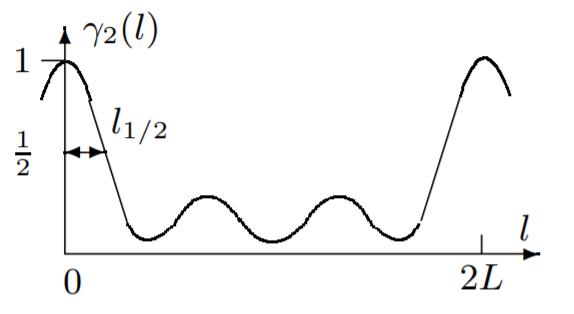
\includegraphics[width=0.4\textwidth]{1.png}
\vspace{-20pt}
\end{center}
\caption{Зависимость $\gamma_2 = \gamma_2(l)$.}
\end{wrapfigure}
$$
\gamma_2 = \dfrac{\sum\limits_n A^2_n \cos \dfrac{2\pi \Delta \nu n l}{c}}{\sum\limits_n A_n^2},
$$
где $l$ – разность хода, $\Delta \nu$ – межмодовое расстояние, $A_n^2$ – интенсивности мод. В непрерывном пределе для гауссовой линии излучения с полушириной $\Delta F$ получаем
$$
\gamma_2 = e^{-\left(\frac{\pi \Delta F l}{c}\right)^2},
$$
при этом полуширина зависимости определяется выражением
\begin{equation}
l_{1/2} = \dfrac{c}{\pi \Delta F}\sqrt{\ln 2} \approx \dfrac{0.26 c}{\Delta F}.
\end{equation}
Функция $\gamma_3$ учитывает разность в поляризации лучей:
\begin{equation}
\gamma_3 = |\cos \alpha|,
\end{equation}
где $\alpha$ – угол между плоскостями поляризаций.

\section{Ход работы}

\subsection{Измерение видности при нулевой разности хода ($\mathcal{V}_2 = 1$)}
При установке нулевой разности хода (при пледе $L = 16$ см) измеряются величины $h_1$, $h_2$, $h_3$ и $h_4$ на экране осциллографа при изменении угла поляризации от $\beta = 0^\circ$ до $\beta = 180^\circ$. Результаты приведены в таблице \ref{t1}.

\begin{longtable}[c]{|c|c|c|c|c|c|c|c|c|c|}
\caption{Измерение видности при нулевой разности хода}
\label{t1}\\
\hline
Угол (°) & 0   & 30  & 50  & 70  & 90  & 110 & 130 & 150 & 180 \\ \hline
\endfirsthead
%
\endhead
%
$h_1$              & 1.0 & 1.5 & 1.5 & 1.6 & 1.2 & 0.7 & 0.5 & 1.1 & 1.2 \\ \hline
$h_2$              & 1.6 & 1.6 & 1.7 & 3.4 & 3.2 & 3.2 & 3.2 & 3.2 & 2.6 \\ \hline
$h_3$              & 0.9 & 1.0 & 1.4 & 3.4 & 3.5 & 2.8 & 3.2 & 2.7 & 1.0 \\ \hline
$h_4$              & 4.2 & 5.1 & 4.8 & 6.2 & 5.7 & 5.1 & 4.4 & 6.0 & 4.7 \\ \hline
\end{longtable}

На основе измеренных значений вычисляется $\mathcal{V}_3$ для каждого случая, после чего строится график зависимости от $\beta$ и проводится сравнение с теоретическими зависимостями $\mathcal{V}_3 = \cos \beta$ и $\mathcal{V}_3 = \cos^2 \beta$. Из-за высокой погрешности измерений график $\mathcal{V}_3(\beta)$, по-видимому, ближе к зависимости $\cos \beta$, что указывает на линейную поляризацию излучения.

\begin{figure}[!h]
\centering
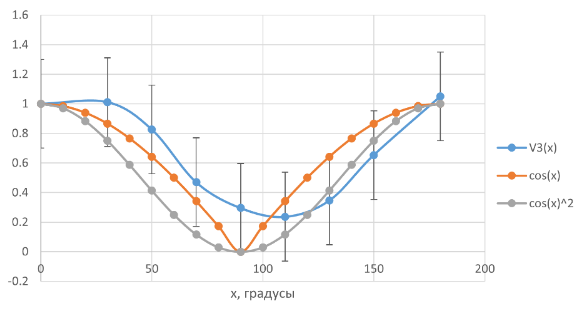
\includegraphics[width=0.8\textwidth]{2.png}
\caption{Зависимость $\mathcal{V}_3(\beta)$}
\label{fig:2}
\end{figure}

\begin{figure}[!h]
\centering
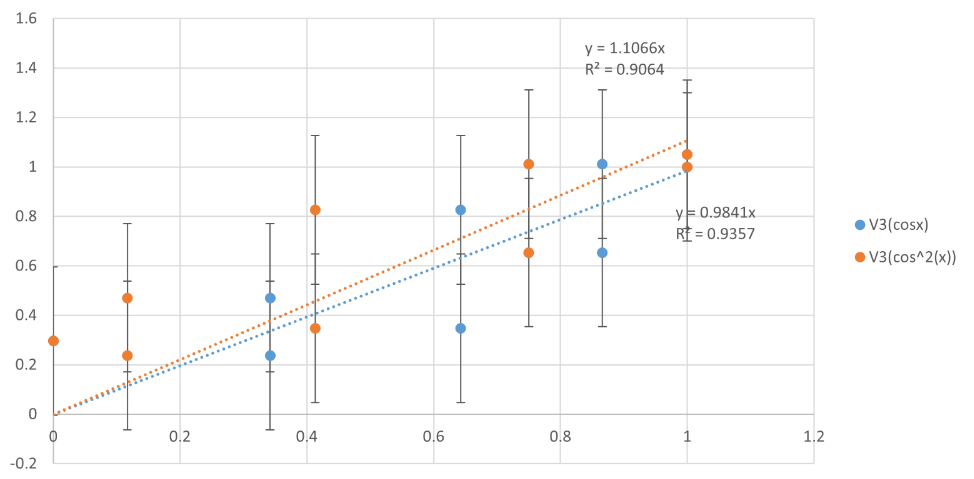
\includegraphics[width=0.8\textwidth]{3.png}
\caption{Зависимость $\mathcal{V}_3(\beta)$}
\label{fig:3}
\end{figure}

\subsection{Измерение видности при постоянном угле поляризации}
При установке оптимального угла поляризации, обеспечивающего максимальную видность, перемещается блок $Б_2$, изменяя разность хода $x$. Аналогичным образом измеряются величины $h_1$, $h_2$, $h_3$ и $h_4$ на экране осциллографа. Результаты фиксируются в таблице, а затем строится график зависимости $\mathcal{V}_2$ от $L$. Параметры $\delta$, $\mathcal{V}$ и $\mathcal{V}_1$ вычисляются по приведённым выше формулам.

\begin{longtable}[c]{|c|c|c|c|c|c|c|c|c|}
\caption{Измерение видности при постоянном угле поляризации}
\label{t2}\\
\hline
L (см) & $h_1$ & $h_2$ & $h_3$ & $h_4$ & $\mathcal{V}$ & $\delta$ & $\mathcal{V}_1$ & $\mathcal{V}_2$ \\ \hline
\endfirsthead
%
\endhead
%
89     & 0.8   & 0.6   & 1     & 2     & 0.33          & 1.33     & 0.99            & 0.34            \\ \hline
78.5   & 1     & 1.2   & 0.9   & 3.6   & 0.60          & 0.83     & 1.00            & 0.60            \\ \hline
84     & 0.8   & 1     & 0.8   & 3     & 0.58          & 0.80     & 0.99            & 0.58            \\ \hline
82     & 0.8   & 1     & 0.6   & 3     & 0.67          & 0.80     & 0.99            & 0.67            \\ \hline
81     & 0.8   & 1.2   & 0.7   & 3.5   & 0.67          & 0.67     & 0.98            & 0.68            \\ \hline
80     & 0.8   & 1.4   & 0.8   & 3.8   & 0.65          & 0.57     & 0.96            & 0.68            \\ \hline
79     & 0.8   & 1.2   & 0.7   & 3.2   & 0.64          & 0.67     & 0.98            & 0.65            \\ \hline
78     & 0.8   & 0.8   & 0.6   & 2.8   & 0.65          & 1.00     & 1.00            & 0.65            \\ \hline
76     & 0.8   & 0.6   & 0.6   & 2.4   & 0.60          & 1.33     & 0.99            & 0.61            \\ \hline
73     & 0.4   & 0.3   & 0.4   & 1.2   & 0.50          & 1.33     & 0.99            & 0.51            \\ \hline
70     & 0.4   & 0.5   & 0.7   & 1.4   & 0.33          & 0.80     & 0.99            & 0.34            \\ \hline
65     & 0.4   & 0.4   & 0.8   & 1     & 0.11          & 1.00     & 1.00            & 0.11            \\ \hline
58     & 1     & 1     & 1.8   & 2.1   & 0.08          & 1.00     & 1.00            & 0.08            \\ \hline
51     & 1     & 1.4   & 2     & 2.9   & 0.18          & 0.71     & 0.99            & 0.19            \\ \hline
45     & 1     & 1.4   & 1.8   & 3     & 0.25          & 0.71     & 0.99            & 0.25            \\ \hline
40     & 1     & 0.7   & 1.6   & 1.8   & 0.06          & 1.43     & 0.98            & 0.06            \\ \hline
35     & 1     & 1.3   & 2     & 2.2   & 0.05          & 0.77     & 0.99            & 0.05            \\ \hline
30     & 1     & 1     & 1.8   & 2.4   & 0.14          & 1.00     & 1.00            & 0.14            \\ \hline
25     & 1     & 0.9   & 1.2   & 2.6   & 0.37          & 1.11     & 1.00            & 0.37            \\ \hline
20     & 1     & 1     & 0.7   & 2.2   & 0.52          & 1.00     & 1.00            & 0.52            \\ \hline
18     & 1     & 0.2   & 0.6   & 1.8   & 0.50          & 5.00     & 0.75            & 0.67            \\ \hline
17     & 1     & 0.4   & 0.4   & 1.2   & 0.50          & 2.50     & 0.90            & 0.55            \\ \hline
16     & 1     & 0.4   & 0.5   & 1.2   & 0.41          & 2.50     & 0.90            & 0.46            \\ \hline
15     & 1     & 0.2   & 0.5   & 1.9   & 0.58          & 5.00     & 0.75            & 0.78            \\ \hline
13     & 1     & 0.3   & 0.6   & 1.2   & 0.33          & 3.33     & 0.84            & 0.40            \\ \hline
10     & 1     & 0.4   & 0.7   & 1     & 0.18          & 2.50     & 0.90            & 0.20            \\ \hline
8      & 1     & 0.2   & 0.8   & 1.6   & 0.33          & 5.00     & 0.75            & 0.45            \\ \hline
\end{longtable}

Построение графика зависимости $\mathcal{V}_2$ от $L$ позволяет сопоставить экспериментальные данные с теоретическими моделями.

\newpage

\begin{figure}[!h]
    \centering
    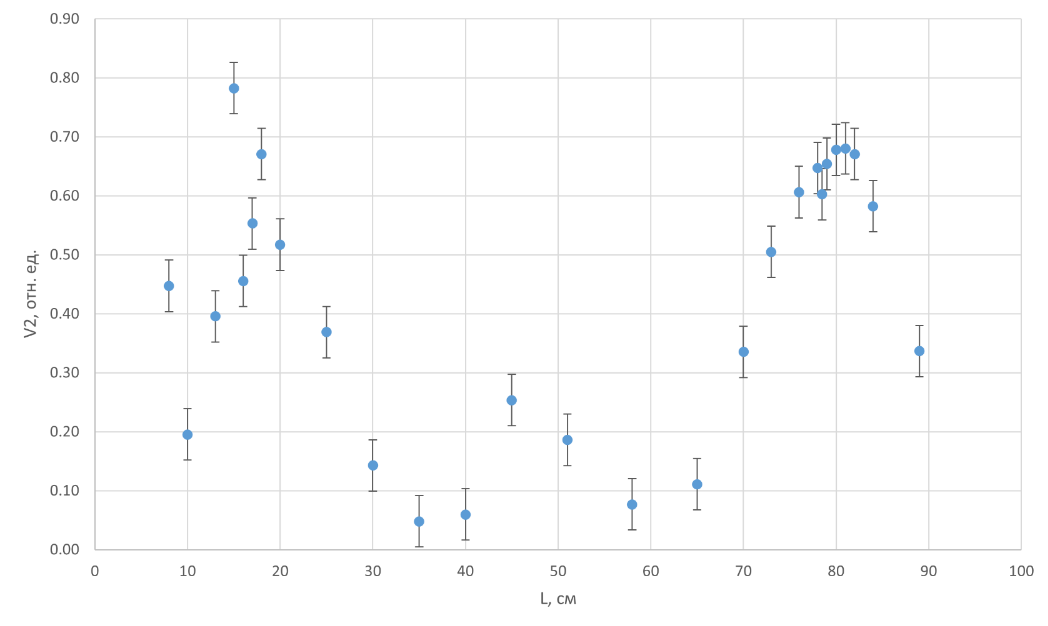
\includegraphics[width=0.6\textwidth]{4.png}
    \caption{Зависимость $\mathcal{V}_2$ от $L$}
\end{figure}

Для определения конфигурации лазера экспериментальные данные сопоставляются с теоретическими зависимостями.

\begin{figure}[!h]
    \centering
    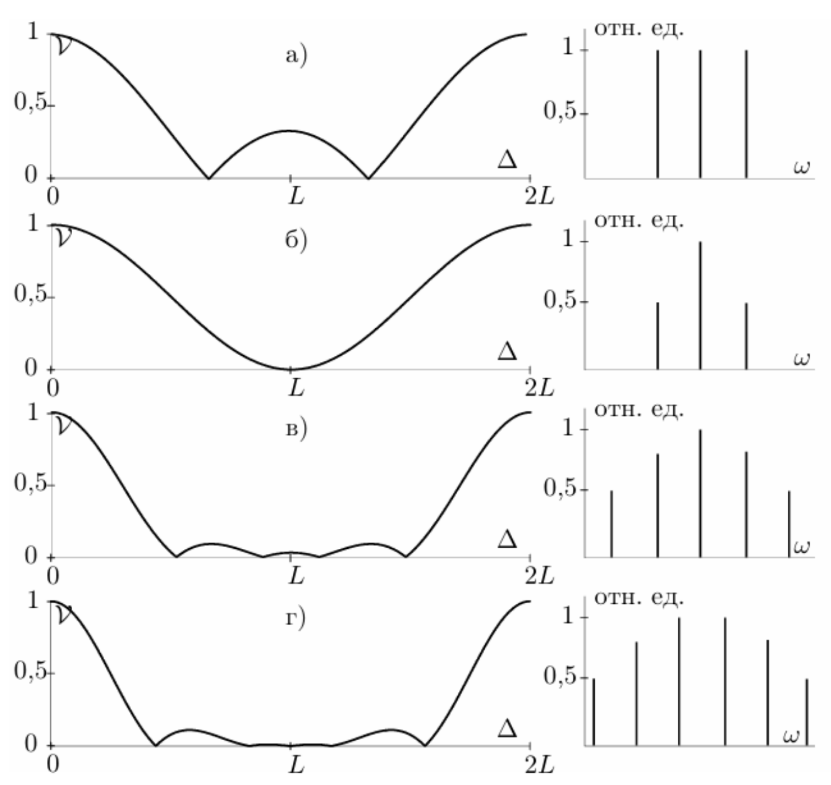
\includegraphics[width=0.6\textwidth]{5.png}
    \caption{Зависимость $\mathcal{V}_2$ от $L$}
\end{figure}

Согласно теории, разность 
\[
\Delta_2 - \Delta_1 = 2L_0,
\]
где $L_0$ — расстояние между зеркалами оптического резонатора лазера. Таким образом,
\[
L_0 = (66 \pm 4) \text{ см.}
\]

Межмодовое расстояние определяется как
\[
\Delta \nu_m = \frac{c}{2L} = (2.27 \pm 0.14) \cdot 10^8 \text{ Гц,}
\]
а полуширина кривой из графика:
\[
l_{1/2} = (10 \pm 3) \text{ см,}
\]
что соответствует разности хода
\[
\Delta_{l1/2} = 2l_{1/2} = (20 \pm 6) \text{ см.}
\]

Наконец, вычислен диапазон частот генерации мод:
\[
\Delta F = \left( 9.0\pm 2.7\right) \cdot 10^8 \text{ Гц,}
\]
а число генерируемых лазером мод:
\[
n = \left( 5\pm 2\right).
\]

\section{Вывод}
Проведённый эксперимент позволил определить спектральные характеристики амплитудной дифракционной решётки, а также оценить угловую дисперсию и разрешающую способность лазерного прибора. В результате были получены следующие значения: расстояние между зеркалами резонатора $L_0 = (66 \pm 4)$ см, межмодовое расстояние $\Delta \nu_m = (2.27 \pm 0.14)\cdot10^8$ Гц, диапазон частот генерации мод $\Delta F = (9.0 \pm 2.7)\cdot10^8$ Гц и число генерируемых мод $n = (5 \pm 2)$. Анализ зависимости видности интерференционной картины от разности хода и поляризации подтвердил, что лазерное излучение имеет линейную поляризацию. Экспериментальные результаты согласуются с теоретическими расчётами, что свидетельствует о корректности используемых моделей, а дальнейшее улучшение точности измерений позволит уточнить полученные значения.

\end{document}
